\documentclass[9pt,aspectratio=169,xcolor=table]{beamer}

%~~~~~~~~~~~~~~~~~~~~~~~~~~~~~~~~~~~~~~~~~~~~~~~~~~~~~~~~~~~~~~~~~~~~~~~~~~~~~~
% Use roboto Font (recommended)
\usepackage[sfdefault]{roboto}
\usepackage[utf8]{inputenc}
\usepackage[T1]{fontenc}
%~~~~~~~~~~~~~~~~~~~~~~~~~~~~~~~~~~~~~~~~~~~~~~~~~~~~~~~~~~~~~~~~~~~~~~~~~~~~~~

%~~~~~~~~~~~~~~~~~~~~~~~~~~~~~~~~~~~~~~~~~~~~~~~~~~~~~~~~~~~~~~~~~~~~~~~~~~~~~~
% Define where theme files are located. ('/styles')
\usepackage{styles/fluxmacros}
\usefolder{styles}
% Use Flux theme v0.1 beta
% Available style: asphalt, blue, red, green, gray
\usetheme[style=hunter]{flux}
%~~~~~~~~~~~~~~~~~~~~~~~~~~~~~~~~~~~~~~~~~~~~~~~~~~~~~~~~~~~~~~~~~~~~~~~~~~~~~~

%~~~~~~~~~~~~~~~~~~~~~~~~~~~~~~~~~~~~~~~~~~~~~~~~~~~~~~~~~~~~~~~~~~~~~~~~~~~~~~
% Extra packages
\usepackage{booktabs}
\usepackage{colortbl}
\usepackage{ragged2e}
\usepackage{amssymb}
\usepackage{multirow}
\usepackage{tikz}
\usetikzlibrary{arrows.meta, positioning, fit, backgrounds, calc, decorations.pathreplacing}
\setbeamertemplate{itemize items}[square]
\usepackage[scaled=.8]{beramono}
\usepackage{listings}
\usepackage{styles/lstlangarm}
\usepackage{array}
\definecolor{bgcolor}{HTML}{F2E9E9}
% lstlangarm.sty references \color{mauve} for string literals but never defines
% it -- only fires when a listing contains a string. Define it here.
\definecolor{mauve}{rgb}{0.58,0,0.82}
% lstlangarm's C style sets commentstyle=green!20, which is unreadable on the
% pink listing background. Darken it globally.
\lstset{commentstyle=\color{green!45!black}}
% ragged-right fixed-width column -- must be defined in the preamble, never
% inside a frame (\newcolumntype's #1 breaks beamer's frame scanner)
\newcolumntype{R}[1]{>{\RaggedRight\arraybackslash}p{#1}}
%~~~~~~~~~~~~~~~~~~~~~~~~~~~~~~~~~~~~~~~~~~~~~~~~~~~~~~~~~~~~~~~~~~~~~~~~~~~~~~
% Table striping: odd rows white, even rows very light gray.
% Needs \documentclass[...,xcolor=table]{beamer} (beamer loads xcolor itself,
% so the option must go on the class, not \usepackage).
\definecolor{stripe}{gray}{0.94}
% \striped makes body rows alternate white, gray, white, ... starting white.
% \rowcolors counts from the first coloured body row; the header is not counted.
\newcommand{\striped}{\rowcolors{1}{white}{stripe}}
%~~~~~~~~~~~~~~~~~~~~~~~~~~~~~~~~~~~~~~~~~~~~~~~~~~~~~~~~~~~~~~~~~~~~~~~~~~~~~~

%~~~~~~~~~~~~~~~~~~~~~~~~~~~~~~~~~~~~~~~~~~~~~~~~~~~~~~~~~~~~~~~~~~~~~~~~~~~~~~
% TikZ block styles -- matches ch1/ch2
% Colour variables are named identically in the book's stm32primer.tex, so any
% tikzpicture using only the \tikzset{...} styles below can be copied verbatim
% between slides and book. Only the \definecolor/\colorlet VALUES differ: the
% book is printed, so it keeps every stroke pure black with muted fills. These
% slides are projected, so both fill AND stroke are bright and saturated to
% grab attention -- see stm32primer.tex for the print palette.
\definecolor{blkfill}{HTML}{DDEEDD}
\definecolor{blkline}{HTML}{355E3B}
\definecolor{accentfill}{HTML}{FFE0B2}
\definecolor{accentline}{HTML}{E65100}
\definecolor{memfill}{HTML}{DFF5DA}
\definecolor{memline}{HTML}{2E7D32}
\definecolor{cellfill}{HTML}{FFFFFF}
\definecolor{cellline}{HTML}{424242}
\definecolor{bitmaskfill}{HTML}{DCEBFF}
\definecolor{bitmaskline}{HTML}{1565C0}
\definecolor{bithitfill}{HTML}{FFE0B2}
\definecolor{bithitline}{HTML}{E65100}
\tikzset{
  blk/.style   = {rectangle, rounded corners=2pt, draw=blkline, fill=blkfill,
                  thick, align=center, font=\small, minimum height=9mm, inner sep=3pt},
  cpublk/.style= {rectangle, rounded corners=2pt, draw=accentline, fill=accentfill,
                  thick, align=center, font=\small\bfseries, minimum height=9mm, inner sep=3pt},
  memblk/.style= {rectangle, rounded corners=2pt, draw=memline, fill=memfill,
                  thick, align=center, font=\small, minimum height=9mm, inner sep=3pt},
  cell/.style  = {rectangle, draw=cellline, fill=cellfill, align=center,
                  font=\small\ttfamily, minimum height=7mm, inner sep=2pt},
  bitcell/.style={rectangle, draw=cellline, fill=cellfill, thick,
                  minimum width=5.4mm, minimum height=5.4mm, inner sep=0pt,
                  font=\scriptsize\ttfamily, anchor=center},
  bitmask/.style={bitcell, fill=bitmaskfill, draw=bitmaskline},
  bithit/.style ={bitcell, fill=bithitfill, draw=bithitline, font=\scriptsize\ttfamily\bfseries},
  rowlab/.style ={font=\scriptsize, text=Gray, anchor=east},
  oplab/.style  ={font=\scriptsize\itshape, text=Gray, anchor=west},
  lbl/.style   = {font=\scriptsize, text=Gray},
  flow/.style  = {-{Stealth[length=2mm]}, thick, draw=blkline},
  busline/.style={thick, draw=cellline},
}
% NOTE (theme quirks -- all fail SILENTLY, always page through the PDF):
%  - a second \\ inside a nested {...} group in a TikZ node breaks parsing
%  - {\small ...} wrapped around a nested itemize eats the frame title + list
%  - \usebeamercolor on a [plain] frame falls through to an unstyled default
%  - \newcolumntype inside a frame breaks beamer's frame scanner
%  - lstlisting needs \begin{frame}[fragile]
%  - a TikZ picture wider than its column silently overflows into neighbours
%~~~~~~~~~~~~~~~~~~~~~~~~~~~~~~~~~~~~~~~~~~~~~~~~~~~~~~~~~~~~~~~~~~~~~~~~~~~~~~

%%%%%%%%%%%%%%%%%%%%%%%%%%%%%%%%%%%
%% BEGIN CONDITIONAL COMPILATION %%
%%%%%%%%%%%%%%%%%%%%%%%%%%%%%%%%%%%
\newif\ifwebex
%\webextrue % uncomment to generate section separator
\ifwebex
\AtBeginSection[]{
  \begin{frame}
  \vfill
  \centering
  \begin{beamercolorbox}[sep=8pt,center,shadow=true,rounded=true]{title}
    \usebeamerfont{title}\insertsectionhead\par%
  \end{beamercolorbox}
  \vfill
  \end{frame}
}
\else
\AtBeginSection[]
{
{
    \setbeamercolor{background canvas}{bg=yellow!10}
    \begin{frame}[plain]
        \frametitle{Table of Contents}
        \tableofcontents[currentsection]
    \end{frame}
}
}
\fi
%%%%%%%%%%%%%%%%%%%%%%%%%%%%%%%%%%%
%% END CONDITIONAL COMPILATION   %%
%%%%%%%%%%%%%%%%%%%%%%%%%%%%%%%%%%%

%~~~~~~~~~~~~~~~~~~~~~~~~~~~~~~~~~~~~~~~~~~~~~~~~~~~~~~~~~~~~~~~~~~~~~~~~~~~~~~
% Information
\title{Boolean Algebra}
\subtitle{\emph{Contemporary Digital Electronic Systems} --- Chapter 5}
\author{Mun\'{i}m Zabidi}
\institute{\color{primary}Faculty of Electrical Engineering, Universiti Teknologi Malaysia}
\date{\today}
\titlegraphic{assets/logoutmwhite.png}
\graphicspath{{.}{../fig/}}
%~~~~~~~~~~~~~~~~~~~~~~~~~~~~~~~~~~~~~~~~~~~~~~~~~~~~~~~~~~~~~~~~~~~~~~~~~~~~~~

\begin{document}

\titlepage

%===============================================================================
\section{Why This Chapter}
%===============================================================================

\begin{frame}{Why This Chapter Matters}
  \begin{columns}[c]
  \begin{column}{.47\textwidth}
    A direct translation of a truth table into gates almost always \alert{wastes gates}. Boolean algebra lets you \emph{simplify} an expression and recover a smaller, faster circuit with the same truth table. It is also the vocabulary of every later design procedure.
  \end{column}
  \begin{column}{.51\textwidth}
    \begin{block}{After this chapter, you can:}
    {\small
    \begin{enumerate}\itemsep2pt
      \item State and apply the laws of Boolean algebra.
      \item Convert between truth tables, expressions and circuits.
      \item Write a function in canonical SOP and POS form.
      \item Simplify an expression algebraically.
      \item Apply De~Morgan's theorems to complement and rewrite expressions.
    \end{enumerate}}
    \end{block}
  \end{column}
  \end{columns}
\end{frame}

\begin{frame}{An Opening Question}
  \leavevmode\vspace{4mm}
  \begin{center}
  \fbox{\parbox{.78\textwidth}{\centering\vspace{2mm}
  \large Why are two circuits with the \alert{same truth table} worth distinguishing?
  \vspace{2mm}}}
  \end{center}
  \vspace{4mm}
  What does ``better'' mean when comparing them? We answer this at the end of the chapter.
\end{frame}

%===============================================================================
\section{Multivariable Theorems}
%===============================================================================

\begin{frame}{Boolean Theorems T1--T14}
  \centering\scriptsize\striped
  \begin{tabular}{@{}rllll@{}}
    \toprule
    & \textbf{Theorem} & \textbf{AND form} & \textbf{OR form} \\
    \midrule
    T1 & Annulment & $A\cdot 0 = 0$ & $A + 1 = 1$ \\
    T2 & Identity & $A\cdot 1 = A$ & $A + 0 = A$ \\
    T3 & Idempotency & $AA = A$ & $A + A = A$ \\
    T4 & Complements & $A\overline{A} = 0$ & $A + \overline{A} = 1$ \\
    T5 & Involution & \multicolumn{2}{c}{$\overline{\overline{A}} = A$} \\
    T6 & Commutative & $AB = BA$ & $A+B = B+A$ \\
    T7 & Associative & $(AB)C = A(BC)$ & $(A+B)+C = A+(B+C)$ \\
    T8 & Distributive & $A(B+C) = AB+AC$ & $A+BC = (A+B)(A+C)$ \\
    T9 & Uniting & $AB+A\overline{B} = A$ & $(A+B)(A+\overline{B}) = A$ \\
    T10 & Absorption & $A+AB = A$ & $A(A+B) = A$ \\
    T11 & Redundancy & $A+\overline{A}B = A+B$ & $(A+\overline{B})B = AB$ \\
    T12 & Consensus & $AB+\overline{A}C = AB+BC+\overline{A}C$ & $(A+B)(\overline{A}+C) = (A+B)(B+C)(\overline{A}+C)$ \\
    T13 & Multiplying & $(A+B)(\overline{A}+C) = AC+\overline{A}B$ & $AB+\overline{A}C = (A+C)(\overline{A}+B)$ \\
    T14 & De Morgan & $\overline{A+B} = \overline{A}\,\overline{B}$ & $\overline{AB} = \overline{A}+\overline{B}$ \\
    \bottomrule
  \end{tabular}
\end{frame}

\begin{frame}{Commutative Law (T6)}
  \centering
  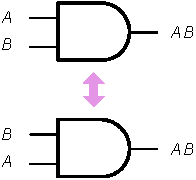
\includegraphics[height=.28\textheight]{boolean-commutative-and}\hspace{8mm}
  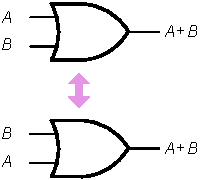
\includegraphics[height=.28\textheight]{boolean-commutative-or}\\[2mm]
  {\small AND \hspace{.3\textwidth} OR}
  \begin{itemize}
    \item Exchanging the inputs of an AND or OR does not change the output: $AB = BA$, $A+B = B+A$.
  \end{itemize}
\end{frame}

\begin{frame}{Associative Law (T7)}
  \centering
  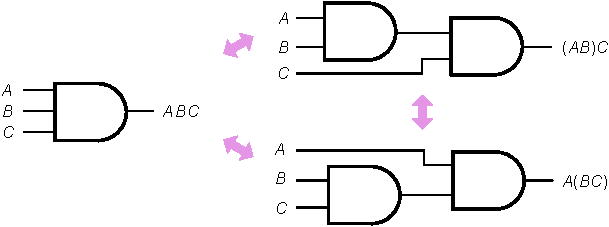
\includegraphics[height=.25\textheight]{boolean-associative-and}\\[2mm]
  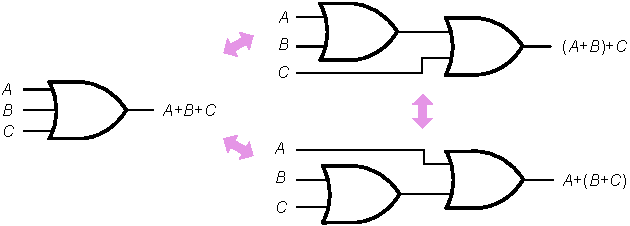
\includegraphics[height=.25\textheight]{boolean-associative-or}
  \begin{itemize}\small
    \item Grouping does not matter when the same operation is used throughout.
    \item Inputs can be reordered or regrouped, which can simplify expressions and circuits.
  \end{itemize}
\end{frame}

\begin{frame}{Proving a Theorem Algebraically}
  \begin{columns}[t]
  \begin{column}{.5\textwidth}
    \begin{block}{Prove $A + AB = A$}
      \small
      \begin{tabular}{rl}
        $A + AB$ & \\
        $= A\cdot 1 + AB$ & identity \\
        $= A(1 + B)$ & distributive \\
        $= A\cdot 1$ & $1 + B = 1$ \\
        $= A$ & identity \\
      \end{tabular}
    \end{block}
  \end{column}
  \begin{column}{.48\textwidth}
    \begin{block}{Prove consensus}
      \scriptsize
      \begin{tabular}{rl}
        $AB + \overline{A}C + BC$ & \\
        $= AB + \overline{A}C + BC(A + \overline{A})$ & complement \\
        $= AB + \overline{A}C + ABC + \overline{A}BC$ & distributive \\
        $= AB(1 + C) + \overline{A}C(1 + B)$ & factoring \\
        $= AB + \overline{A}C$ & identity \\
      \end{tabular}
    \end{block}
  \end{column}
  \end{columns}
\end{frame}

%===============================================================================
\section{De Morgan's Theorems}
%===============================================================================

\begin{frame}{De Morgan's Theorems}
  \begin{columns}[c]
  \begin{column}{.5\textwidth}
    \begin{block}{The two theorems}
      \[ \overline{A \cdot B} = \overline{A} + \overline{B} \]
      \[ \overline{A + B} = \overline{A} \cdot \overline{B} \]
    \end{block}
    \begin{itemize}\small\itemsep2pt
      \item Break the long bar; the operation under the break \alert{changes} (AND to OR, OR to AND).
      \item Valid for any number of variables.
    \end{itemize}
  \end{column}
  \begin{column}{.48\textwidth}
    \centering
    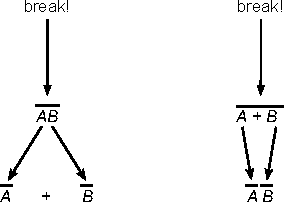
\includegraphics[width=\textwidth]{demorgan}
  \end{column}
  \end{columns}
  \small
  \[ \overline{ABC} = \overline{A} + \overline{B} + \overline{C} \qquad \overline{A+BC} = \overline{A}\,(\overline{B} + \overline{C}) \]
\end{frame}

\begin{frame}{De Morgan Changes the Gate}
  \centering
  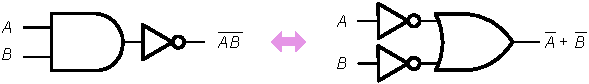
\includegraphics[height=.22\textheight]{demorgan-and}\\[4mm]
  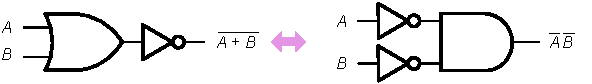
\includegraphics[height=.22\textheight]{demorgan-or}
  \begin{itemize}\small
    \item An AND gate can be redrawn as an OR gate by adding and removing inverters, and vice versa.
  \end{itemize}
\end{frame}

%===============================================================================
\section{Expressing Logic Circuits}
%===============================================================================

\begin{frame}{SOP and POS Forms}
  \begin{columns}[t]
  \begin{column}{.5\textwidth}
    \begin{block}{Sum-of-products (SOP)}
      \small AND terms combined by OR: an \alert{AND-OR} network.\\
      $F = AB + \overline{A}C$
    \end{block}
  \end{column}
  \begin{column}{.48\textwidth}
    \begin{block}{Product-of-sums (POS)}
      \small OR terms combined by AND: an \alert{OR-AND} network.\\
      $F = (A+B)(\overline{A}+C)$
    \end{block}
  \end{column}
  \end{columns}
  \vspace{2mm}
  \begin{itemize}\small\itemsep2pt
    \item POS to SOP: multiply out the terms and simplify.
    \item SOP to POS: use De Morgan's theorems with involution, $\overline{\overline{A}} = A$.
    \item SOP is slightly more convenient.
  \end{itemize}
\end{frame}

\begin{frame}{Converting Between SOP and POS}
  \begin{columns}[t]
  \begin{column}{.46\textwidth}
    \begin{block}{$(A+C)(B+\overline{C})$ to SOP}
      \small
      $= AB + A\overline{C} + BC + C\overline{C}$\\
      $= AB + A\overline{C} + BC$
    \end{block}
  \end{column}
  \begin{column}{.52\textwidth}
    \begin{block}{$F = A\overline{B} + B\overline{C}$ to POS}
      \scriptsize
      $\overline{F} = (\overline{A}+B)(\overline{B}+C) = \overline{A}\,\overline{B} + \overline{A}C + BC$\\[1mm]
      $F = \overline{\overline{F}} = (A+B)(A+\overline{C})(\overline{B}+\overline{C})$
    \end{block}
  \end{column}
  \end{columns}
  \vspace{2mm}
  {\small Method: complement with De Morgan, expand to SOP, then apply De Morgan again.}
\end{frame}

\begin{frame}{Expression to Circuit}
  \begin{columns}[c]
  \begin{column}{.5\textwidth}
    \small
    $F = A\overline{B}C + \overline{A}B + ABC + \overline{A}C$
    \begin{itemize}\itemsep2pt
      \item 3 variables, 4 product terms, 10 literals.
      \item Each AND needs an AND gate, each OR an OR gate, each complement a NOT.
      \item Gate inputs: $10 + 4 = 14$ (excluding inverters).
    \end{itemize}
  \end{column}
  \begin{column}{.48\textwidth}
    \centering
    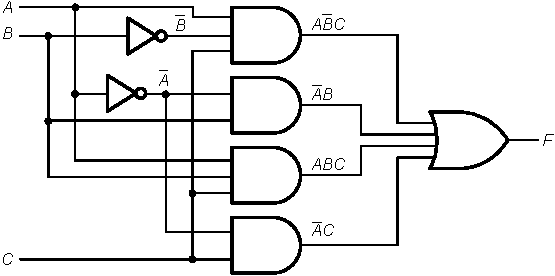
\includegraphics[width=\textwidth]{boolean-firstnet}
  \end{column}
  \end{columns}
  \vspace{2mm}
  {\small Simplification reduces literals and gate inputs: less power and shorter delay.}
\end{frame}

\begin{frame}{Circuit to Expression}
  \begin{columns}[c]
  \begin{column}{.42\textwidth}
    \centering
    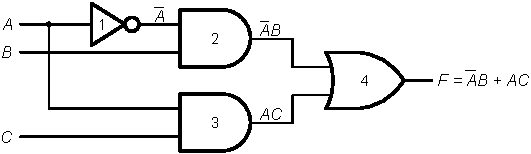
\includegraphics[width=\textwidth]{boolean-secondnet}
  \end{column}
  \begin{column}{.56\textwidth}
    \begin{enumerate}\small\itemsep2pt
      \item Name all gate inputs.
      \item Write each gate's expression at its output, left to right.
      \item The last gate's output is the network equation.
    \end{enumerate}
    \small Gate 1: $\overline{A}$. Gate 2: $\overline{A}B$. Gate 3: $AC$.\\
    Gate 4: $F = \overline{A}B + AC$.
  \end{column}
  \end{columns}
\end{frame}

\begin{frame}{Truth Table of a Network}
  \centering\footnotesize\striped
  \begin{tabular}{ccc|c|c|c||c}
    \toprule
    $A$ & $B$ & $C$ & $\overline{A}$ & $\overline{A}B$ & $AC$ & $F$ \\
    \midrule
    0 & 0 & 0 & 1 & 0 & 0 & 0 \\
    0 & 0 & 1 & 1 & 0 & 0 & 0 \\
    0 & 1 & 0 & 1 & 1 & 0 & 1 \\
    0 & 1 & 1 & 1 & 1 & 0 & 1 \\
    1 & 0 & 0 & 0 & 0 & 0 & 0 \\
    1 & 0 & 1 & 0 & 0 & 1 & 1 \\
    1 & 1 & 0 & 0 & 0 & 0 & 0 \\
    1 & 1 & 1 & 0 & 0 & 1 & 1 \\
    \bottomrule
  \end{tabular}
  \begin{itemize}\small
    \item Columns for every input, every gate output, and the final output; fill the gates in order.
  \end{itemize}
\end{frame}

%===============================================================================
\section{Canonical Forms}
%===============================================================================

\begin{frame}{Why Canonical Forms?}
  \begin{itemize}
    \item A truth table is a \alert{unique} description of a function. Expressions and circuits are not.
    \item Two different-looking expressions may give identical outputs for every input.
    \item A \alert{canonical form} writes a function uniquely and systematically from its truth table.
  \end{itemize}
  \begin{center}
  \small\striped
  \begin{tabular}{lcc}
    \toprule
    \textbf{Canonical form} & \textbf{Structure} & \textbf{Built from} \\
    \midrule
    SOP & OR of AND terms & minterms \\
    POS & AND of OR terms & maxterms \\
    \bottomrule
  \end{tabular}
  \end{center}
\end{frame}

\begin{frame}{Minterms and Maxterms}
  \begin{columns}[c]
  \begin{column}{.5\textwidth}
    \begin{itemize}\small\itemsep3pt
      \item \alert{Minterm}: an AND of all variables, each once, true or complemented. It is 1 for exactly \alert{one} input row.
      \item \alert{Maxterm}: an OR of all variables, each once. It is 0 for exactly \alert{one} input row.
      \item $A\overline{B}C$ is a minterm; $A\overline{B}$ is not (missing $C$).
    \end{itemize}
  \end{column}
  \begin{column}{.48\textwidth}
    \centering\scriptsize\striped
    \begin{tabular}{@{}ccc|ll@{}}
      \toprule
      $A$ & $B$ & $C$ & Minterm & Maxterm \\
      \midrule
      0 & 0 & 0 & $m_0=\overline{A}\,\overline{B}\,\overline{C}$ & $M_0=A+B+C$ \\
      0 & 0 & 1 & $m_1=\overline{A}\,\overline{B}C$ & $M_1=A+B+\overline{C}$ \\
      0 & 1 & 0 & $m_2=\overline{A}B\overline{C}$ & $M_2=A+\overline{B}+C$ \\
      0 & 1 & 1 & $m_3=\overline{A}BC$ & $M_3=A+\overline{B}+\overline{C}$ \\
      1 & 0 & 0 & $m_4=A\overline{B}\,\overline{C}$ & $M_4=\overline{A}+B+C$ \\
      1 & 0 & 1 & $m_5=A\overline{B}C$ & $M_5=\overline{A}+B+\overline{C}$ \\
      1 & 1 & 0 & $m_6=AB\overline{C}$ & $M_6=\overline{A}+\overline{B}+C$ \\
      1 & 1 & 1 & $m_7=ABC$ & $M_7=\overline{A}+\overline{B}+\overline{C}$ \\
      \bottomrule
    \end{tabular}
  \end{column}
  \end{columns}
\end{frame}

\begin{frame}{Canonical SOP from a Truth Table}
  \begin{columns}[c]
  \begin{column}{.4\textwidth}
    \centering\small
    \begin{tabular}{ccc|cl}
      \toprule
      $A$ & $B$ & $C$ & $F$ & \\
      \midrule
      0 & 0 & 0 & 1 & $m_0$ \\
      0 & 0 & 1 & 0 & \\
      0 & 1 & 0 & 1 & $m_2$ \\
      0 & 1 & 1 & 0 & \\
      1 & 0 & 0 & 0 & \\
      1 & 0 & 1 & 0 & \\
      1 & 1 & 0 & 1 & $m_6$ \\
      1 & 1 & 1 & 1 & $m_7$ \\
      \bottomrule
    \end{tabular}
  \end{column}
  \begin{column}{.58\textwidth}
    \begin{itemize}\small\itemsep3pt
      \item Pick the rows where $F = 1$; write each row's minterm; OR them.
    \end{itemize}
    \[ F = \overline{A}\,\overline{B}\,\overline{C} + \overline{A}B\overline{C} + AB\overline{C} + ABC \]
    \[ F(A,B,C) = \sum m(0,2,6,7) \]
  \end{column}
  \end{columns}
\end{frame}

\begin{frame}{Expanding to Canonical SOP}
  \begin{itemize}\small\itemsep2pt
    \item For each missing variable $X$, multiply the term by $(X + \overline{X}) = 1$ and expand. Drop duplicate terms.
    \item Canonical forms also let you compare expressions: equal expressions have equal minterm lists.
  \end{itemize}
  \begin{columns}[t]
  \begin{column}{.48\textwidth}
    \begin{block}{$F = AB$}
      \small
      $= AB(C + \overline{C}) = ABC + AB\overline{C}$\\
      $= \sum m(6,7)$
    \end{block}
  \end{column}
  \begin{column}{.5\textwidth}
    \begin{block}{$F = A + B\overline{C}$}
      \small
      $= A(B+\overline{B})(C+\overline{C}) + B\overline{C}(A+\overline{A})$\\
      $= \sum m(2,4,5,6,7)$
    \end{block}
  \end{column}
  \end{columns}
\end{frame}

\begin{frame}{Proving Equivalence with Canonical Forms}
  \begin{block}{Prove $AB + \overline{A}C = (\overline{A}+B)(A+C)$}
    \small
    LHS $= AB(C+\overline{C}) + \overline{A}C(B+\overline{B}) = m_6 + m_7 + m_1 + m_3 = \sum m(1,3,6,7)$\\[2mm]
    RHS $= \overline{A}C + AB + BC$, expanded: $m_1 + m_3 + m_6 + m_7 = \sum m(1,3,6,7)$\\[2mm]
    Both give $\sum m(1,3,6,7)$, so the expressions are equal.
  \end{block}
\end{frame}

\begin{frame}{Canonical POS}
  \begin{columns}[c]
  \begin{column}{.4\textwidth}
    \centering\small
    \begin{tabular}{ccc|cl}
      \toprule
      $A$ & $B$ & $C$ & $F$ & \\
      \midrule
      0 & 0 & 0 & 1 & \\
      0 & 0 & 1 & 0 & $M_1$ \\
      0 & 1 & 0 & 1 & \\
      0 & 1 & 1 & 0 & $M_3$ \\
      1 & 0 & 0 & 0 & $M_4$ \\
      1 & 0 & 1 & 0 & $M_5$ \\
      1 & 1 & 0 & 1 & \\
      1 & 1 & 1 & 1 & \\
      \bottomrule
    \end{tabular}
  \end{column}
  \begin{column}{.58\textwidth}
    \begin{itemize}\small\itemsep3pt
      \item Pick the rows where $F = 0$; write each row's maxterm; AND them.
    \end{itemize}
    \small
    $F = (A+B+\overline{C})(A+\overline{B}+\overline{C})(\overline{A}+B+C)(\overline{A}+B+\overline{C})$
    \[ F(A,B,C) = \prod M(1,3,4,5) \]
    \begin{itemize}\small
      \item To add a missing variable $C$ to a sum term: $A + B = (A+B+C)(A+B+\overline{C})$.
    \end{itemize}
  \end{column}
  \end{columns}
\end{frame}

\begin{frame}{Converting Between Canonical Forms}
  \begin{itemize}\small\itemsep3pt
    \item A function is 1 at its minterm indices and 0 at its maxterm indices.
    \item The two index lists are \alert{complementary}: swap to the indices that are missing.
  \end{itemize}
  \begin{columns}[t]
  \begin{column}{.48\textwidth}
    \begin{block}{SOP to POS}
      \small $F = \sum m(3,4,5,6,7)$. Missing indices: 0, 1, 2.\\
      $F = \prod M(0,1,2)$
    \end{block}
  \end{column}
  \begin{column}{.5\textwidth}
    \begin{block}{POS to SOP}
      \small $F = \prod M(1,2,5)$. Missing indices: 0, 3, 4, 6, 7.\\
      $F = \sum m(0,3,4,6,7)$
    \end{block}
  \end{column}
  \end{columns}
\end{frame}

%===============================================================================
\section{Don't Cares}
%===============================================================================

\begin{frame}{Incompletely Specified Functions}
  \begin{columns}[c]
  \begin{column}{.5\textwidth}
    \centering
    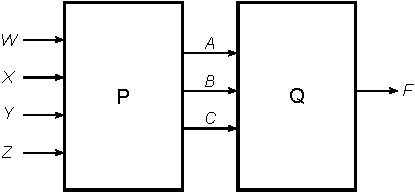
\includegraphics[width=\textwidth]{incompletelyspecified}
  \end{column}
  \begin{column}{.25\textwidth}
    \centering\small
    \begin{tabular}{ccc|c}
      \toprule
      $A$ & $B$ & $C$ & $F$ \\
      \midrule
      0 & 0 & 0 & 1 \\
      0 & 0 & 1 & 1 \\
      0 & 1 & 0 & 0 \\
      0 & 1 & 1 & 0 \\
      1 & 0 & 0 & 0 \\
      1 & 0 & 1 & 1 \\
      1 & 1 & 0 & $\times$ \\
      1 & 1 & 1 & $\times$ \\
      \bottomrule
    \end{tabular}
  \end{column}
  \begin{column}{.23\textwidth}
    \small
    $F = \sum m(0,1,5) + \sum d(6,7)$\\[2mm]
    $F = \prod M(2,3,4)\prod D(6,7)$
  \end{column}
  \end{columns}
  \vspace{2mm}
  \begin{itemize}\small
    \item Some input combinations never occur, or the output does not matter. These are \alert{don't cares}, written $\times$, $-$ or $.$
    \item Assign them 0 or 1 freely to simplify the function and cut gates.
  \end{itemize}
\end{frame}

%===============================================================================
\section{Algebraic Simplification}
%===============================================================================

\begin{frame}{Simplification Procedure}
  \centering\small\striped
  \begin{tabular}{@{}cR{.2\textwidth}ll@{}}
    \toprule
    \textbf{Step} & \textbf{Action} & \textbf{Before} & \textbf{After} \\
    \midrule
    1 & Convert to SOP & $(A+B)(C+D)$ & $AC+AD+BC+BD$ \\
    2 & Drop exact duplicates & $A\overline{B}+CB+A\overline{B}$ & $A\overline{B}+CB$ \\
    3 & Drop null terms & $A(\overline{A}+B)$ & $A\overline{A}+AB = AB$ \\
    4 & Absorb contained terms & $AB+ABC$ & $AB(1+C) = AB$ \\
    5 & Combine terms differing in one literal & $ABC+AB\overline{C}$ & $AB(C+\overline{C}) = AB$ \\
    \bottomrule
  \end{tabular}
\end{frame}

\begin{frame}{Simplification Examples}
  \begin{columns}[t]
  \begin{column}{.5\textwidth}
    \begin{block}{$F = (A+B)(A+\overline{B})(\overline{A}+C)$}
      \scriptsize
      $= [A + A(\overline{B}+B) + 0](\overline{A}+C)$\\
      $= A(\overline{A}+C) = A\overline{A} + AC$\\
      $= AC$
    \end{block}
    \begin{block}{$F = \overline{A}B + A\overline{B}C + BC$}
      \scriptsize
      $= \overline{A}B + (A\overline{B}+B)C = \overline{A}B + (A+B)C$\\
      $= \overline{A}B + AC + BC = \overline{A}B + AC$
    \end{block}
  \end{column}
  \begin{column}{.48\textwidth}
    \begin{block}{$F = AB + \overline{A}C + BC$}
      \scriptsize
      $= AB + \overline{A}C + BC(A+\overline{A})$\\
      $= A(B+BC) + \overline{A}(C+BC)$\\
      $= AB + \overline{A}C$\\
      This proves the consensus theorem.
    \end{block}
    \begin{block}{$F = \overline{(A+\overline{B})(\overline{C}+D)}$ to SOP}
      \scriptsize
      $= \overline{(A+\overline{B})} + \overline{(\overline{C}+D)}$\\
      $= \overline{A}B + C\overline{D}$
    \end{block}
  \end{column}
  \end{columns}
\end{frame}

\begin{frame}{Back to the Opening Question}
  \begin{block}{What makes one circuit ``better''?}
    \begin{itemize}\small\itemsep3pt
      \item Fewer \alert{literals} and \alert{gate inputs}: less area and cost.
      \item Fewer gates in the path: shorter \alert{delay}.
      \item Less switching hardware: lower \alert{power}.
    \end{itemize}
  \end{block}
  Boolean algebra gets us from the first, correct-but-large expression to a smaller one with the same truth table.
\end{frame}

%===============================================================================
\section{Summary}
%===============================================================================

\begin{frame}{Summary}
  \begin{itemize}\itemsep3pt\small
    \item A function can be a truth table, an expression or a circuit: all carry the same information.
    \item \alert{Canonical SOP} is a sum of minterms; \alert{canonical POS} is a product of maxterms, dual to SOP.
    \item \alert{De Morgan's theorems} link AND with OR under complementation.
    \item \alert{Don't cares} let you simplify further.
    \item Algebraic simplification is systematic but error-prone by hand.
  \end{itemize}
  \begin{block}{Looking ahead}
    Chapter 6 introduces Karnaugh maps, a visual tool that automates minimisation.
  \end{block}
\end{frame}

\end{document}
